\section{Processes}

\subsection{Interaction as developers}
% How do you interact as developers?
% How is the team organized?

\subsection{Tools and stages included in CI/CD pipelines}
\label{tools-and-stages-ci-cd}
% A complete description of stages and tools included in the CI/CD chains.
% That is, including deployment and release of your systems.
Our CI/CD pipelines are implemented using Github Actions. Our workflows are splitted in the following:

\subsubsection{quality.yml}
Triggered on pull request actions (opened, reopened, edited, synchronize, and ready for review). The main purpose is to run quality checks over the changes existing on the pull request branch.

\begin{itemize}
    \item .NET SDK (for running dotnet commands)
    \item Hadolint (for Dockerfile linting)
    \item SonarQube (for code quality and security analysis)
\end{itemize}

\subsubsection{release.yml}
Triggered on pushes to \texttt{main} branch. It uses a base \texttt{release.config.js} file at the root of the repository and it is meant to automate the generation of releases and its changelogs through the use of conventional commit messages.
\begin{itemize}
    \item Node.js (for running npm and semantic-release)
    \item Semantic Release (for versioning and changelog management)
\end{itemize}

\subsubsection{deploy.yml}
Triggered on pushes to \texttt{develop} and \texttt{main}. It internally checks the targeted environment \texttt{(staging} or \texttt{prod)} retrieving the corresponding secrets,pushing the application image to Dockerhub and deploying to Digital Ocean.
\begin{itemize}
    \item Docker (login, build, push actions)
    \item SSH (for deploying to servers)
\end{itemize}

\subsection{Organization of the repository}
% Organization of your repositor(ies).
% That is, either the structure of of mono-repository or organization of artifacts across repositories.
% In essence, it has to be be clear what is stored where and why.
The repository is organised in two main folders: csharp-minitwit and infrastructure. The first contains all application specific logic, while the second holds all infrastructure related configuration files.

By organising the repository in this manner, there is a clear separation of concerns, making it easier to manage the project. Developers concerning with the development of the application do not need to understand the intricacies of the infrastructure and vice versa. 

\subsubsection{csharp-minitwit}
Main folders and files explained:
\begin{itemize}
    \item Controllers: APIController and HomeController handle all the logic for each endpoint.
    \item Databases: contains the \texttt{schema.sql} and \texttt{minitwit.db} files used to initialise the database in the development environment.
    \item Metrics: contain all metrics logic and configuration.
    \item Middlewares: currently only a CatchAllMiddleware required to catch incoming requests and record metrics.
    \item Models: these represent the way the data is shaped in the application. %I do not completely understand the division into api and DTOs. We should probably explain why.
    \item Services: include the business logic and service layer components. ORM logic is reflected under Repositories.
    \item Views: templates representing the user interface.
\end{itemize}

\subsubsection{infrastructure}
Main folders and files explained:
\begin{itemize}
    \item archive
    \item grafana
    \item scripts
    \item ssh\_key
    \item stack
\end{itemize}
    
    
\subsection{Applied branching strategy}
We have decided to use Gitflow branching model\cite{nvie2010git}. In this model the repository holds two main branches:
\begin{itemize}
    \item \texttt{main}: represents the main branch where the source code of HEAD is always production-ready.
    \item \texttt{develop}: it serves as an integration branch where source code of HEAD always reflects a state with the latest delivered development changes for the next release.
\end{itemize}
Next to these main branches there are some other supporting branches, being \texttt{feature} the most widely used. feature branches are meant to be used to develop new features for future releases. They usually branch off and back to develop.

\subsection{Applied development process and tools supporting it}
% For example, how did you use issues, Kanban boards, etc. to organize open tasks
To organise the development process and make work visible we decided to capitalise Github's built in Project tab, which provides an adaptable spreadsheet for tracking work, and which also integrates with Issues and Pull Requests. This tool provides a comprehensive visibility to the current state of each ticket and an easy-to-understand interface for developers and stakeholders.

A new Issue is created to document a new requirement and is automatically shown in the Project board as a "Todo" item. When a team member is assigned to such issue, it is moved into the "In Progress" state. The development phase takes part, and when the issue is closed, it is automatically moved to the "Done" status in the board. Closing an issue as "not planned" takes the ticket to the "Aborted" status.

\begin{figure}[H]
    \centering
    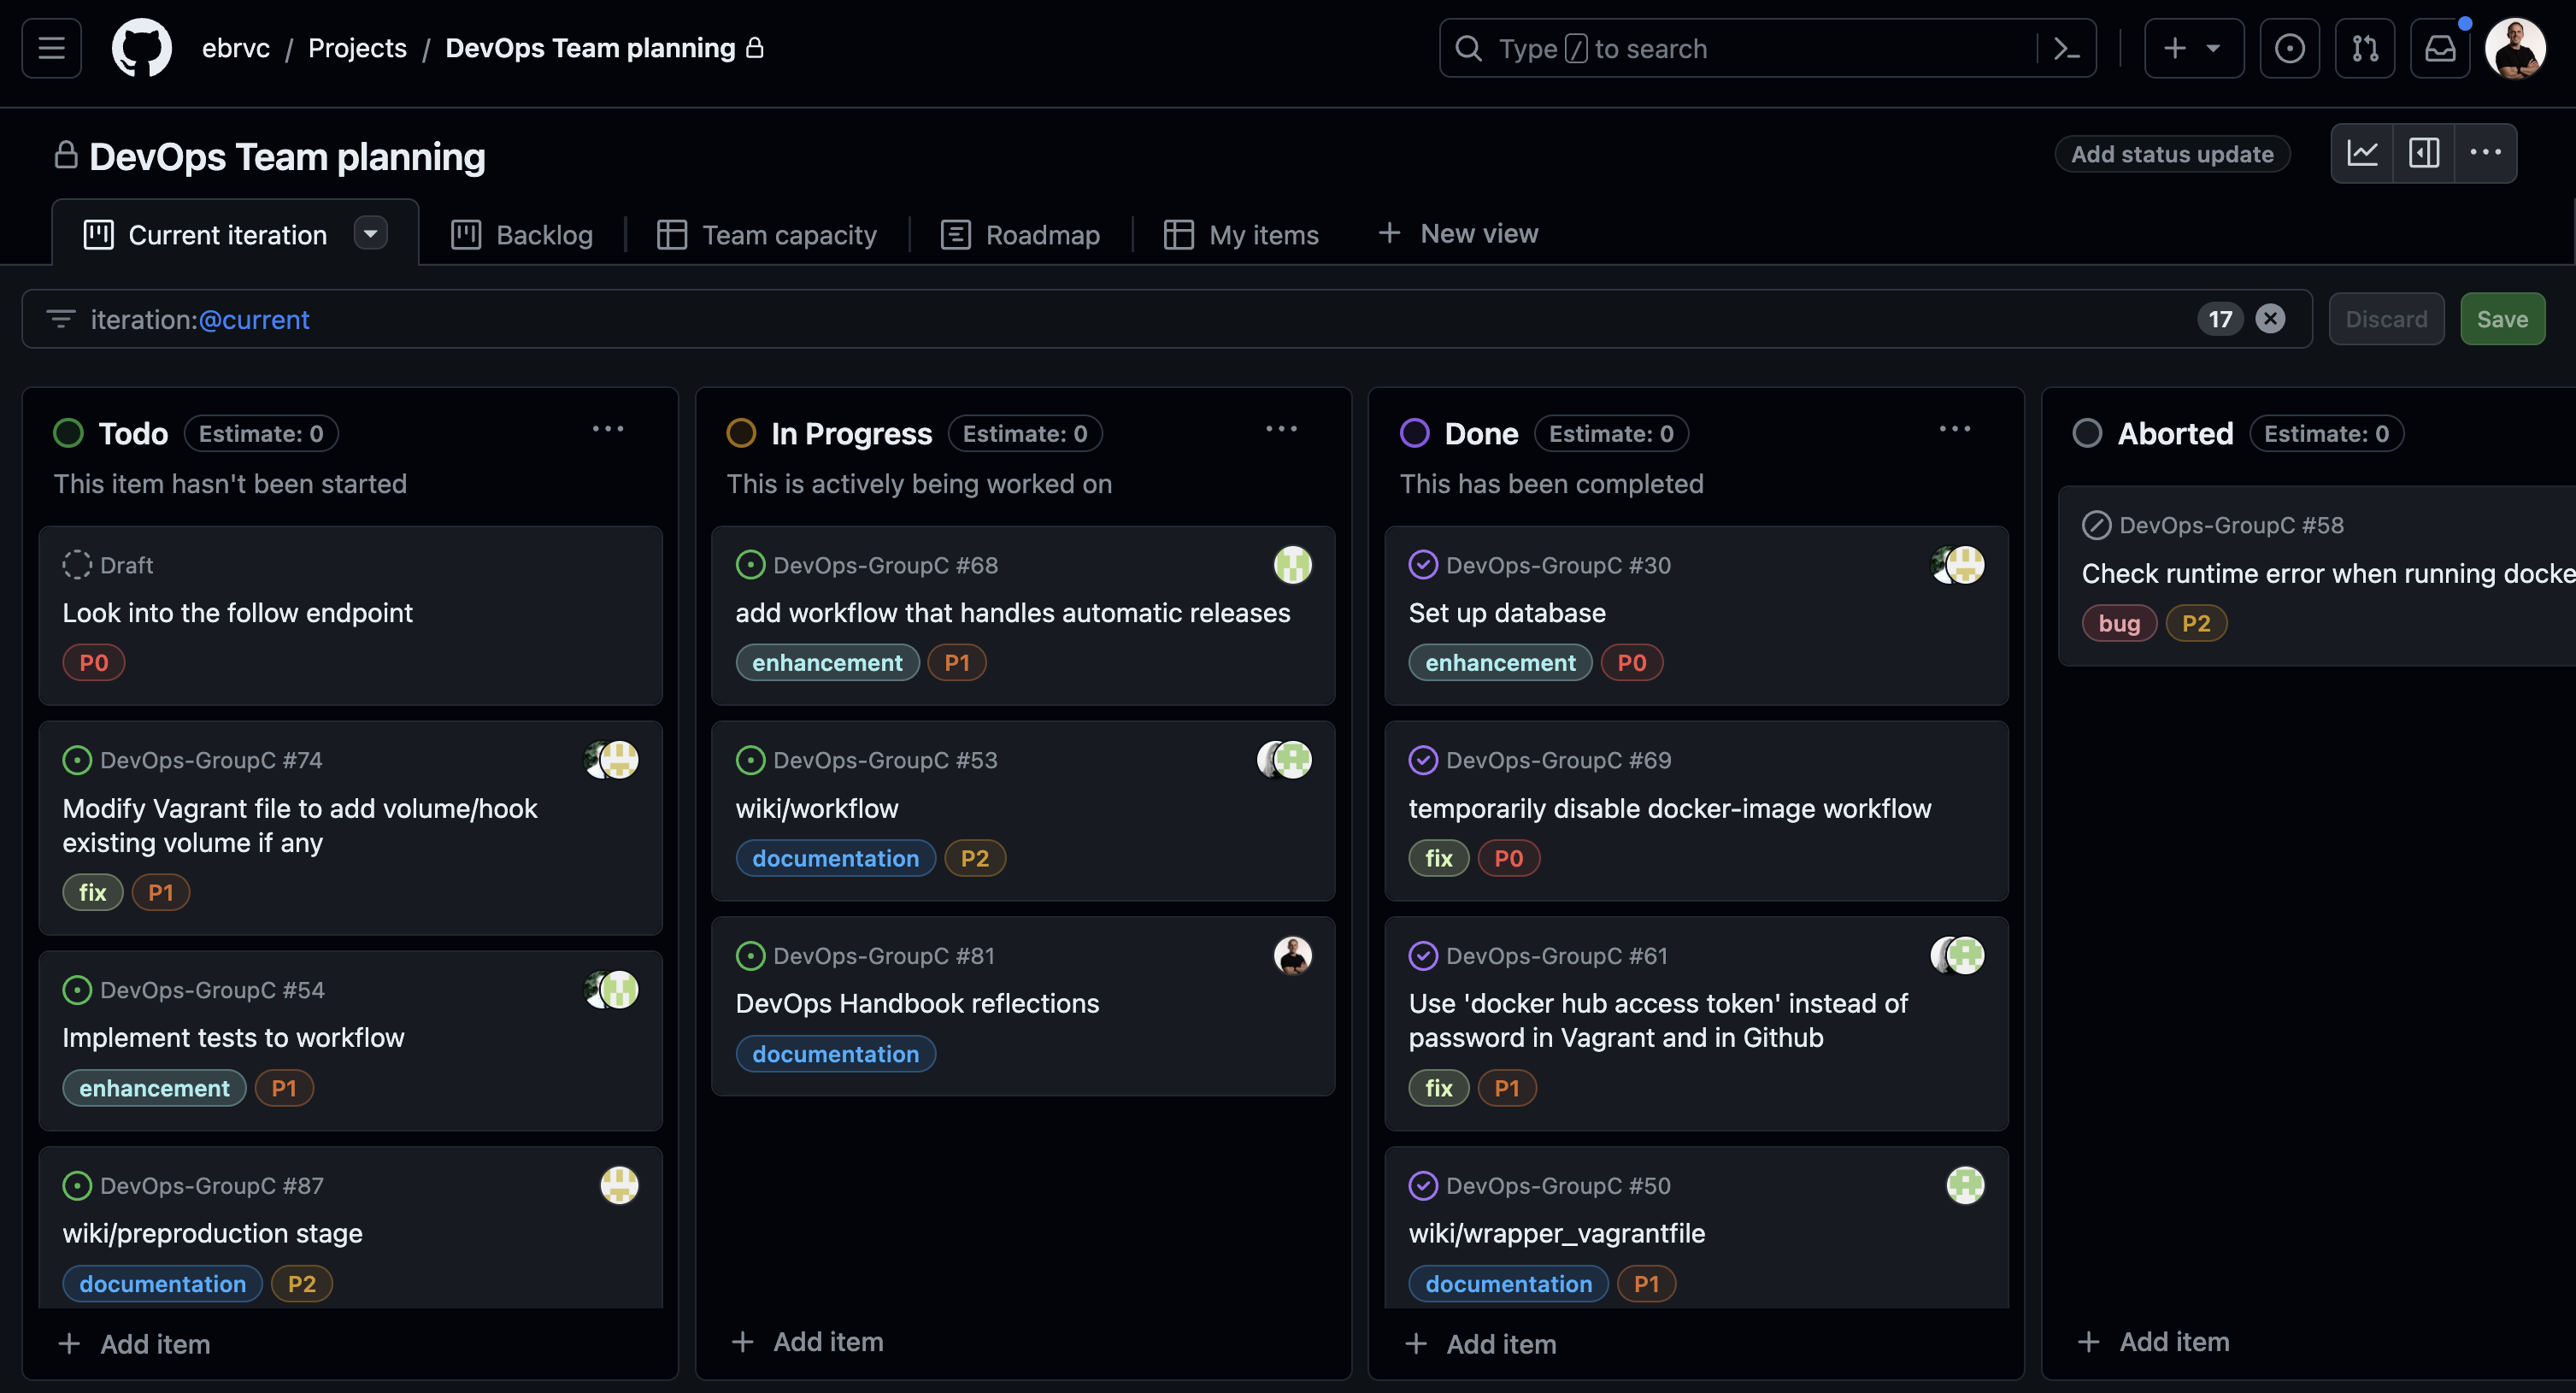
\includegraphics[width=\textwidth]{images/github-project-tracking.png}
    \caption{Github's Project tracking tool}
    \label{fig:github-project-feature}
\end{figure}

\subsection{Monitoring and logging}
% How do you monitor your systems and what precisely do you monitor?
% What do you log in your systems and how do you aggregate logs?
Monitoring is done through a self hosted image of Grafana using a Digital Ocean Droplet that receives the metrics data from Prometheus servers attached to the application droplets. Moreover, logging is configured through a log aggregation system called Loki, which acts as a Grafana datasource. These logs are pushed directly to Loki by using Serilog, a logging library for .NET applications.

\subsubsection{Monitoring the business}
These metrics are registered by querying the database on some specific indicators, such as:
\begin{itemize}
    \item Messages registered (application usage)
    \item Users registered (conversion)
    \item Follower registrations (users interaction level)
\end{itemize}

\subsubsection{Application monitoring}
\begin{itemize}
    \item Rate of HTTP requests received per endpoint
    \item Total number of requests (last 24hs)
    \item Total count of errors per status code (last 24hs).
    \item Top 10 unhandled exception endpoints.
    \item Top 10 Requested endpoints (API).
\end{itemize}

\subsection{Application logging}
The reason why we have chosen Loki as a logging mechanism is due to its inherent simpler architecture. It requires less computational power and memory, this aligns perfectly with our MiniTwit application.
Below, we present the log events throughout our application:
\begin{itemize}
    \item Message posting
    \item User logging / Failure logging / Invalid username or password
    \item User logout
    \item User registering / Failure registering
    \item API requests that are not from the simulator
    \item API registering / Failure registering
    \item API message posting from users / Failure or incorrect usage of endpoint
    \item API retrieval of messages for a specific user / Failure in the retrieval
    \item API retrieval of followers for a specific user / Failure in the retrieval
    \item API follow/unfollow requests / Failure in the execution
    
\end{itemize}

\subsubsection{Infrastructure monitoring}
Even though we haven't set this monitoring ourselves, Digital Ocean provides some out of the box monitoring for its droplets, such as CPU usage, memory usage, DISK I/O, Disk Usage, Bandwith, etc.
\todo{Describe how we aggregate logs}

\subsection{Security assessment}
Brief results of the security assessment.


\subsection{Scaling and upgrades}
Because we monitor our system we can see when there would be a need to scale our system up or down. Our strategy for scaling our system is to change the number of nodes in the terraform file minitwit\textunderscore swarm\textunderscore cluster.tf and run the bootstrap.sh script. Because the state of our system is kept in the Spaces Object Storage in DigitalOcean it would allow for a quick scaling of the number of nodes. 
\todo{Describe our strategy for upgrades}
%Applied strategy for scaling and load balancing.
%In essence it has to be clear how code or other artifacts come from idea into the running system and everything that happens on the way.
% Applied strategy for scaling and upgrades